\documentclass{standalone}

\usepackage[OT1]{fontenc}
\renewcommand*\familydefault{\sfdefault}
\usepackage{helvet,sfmath}
\usepackage{siunitx}

\usepackage{tikz}
\usetikzlibrary{arrows,calc,patterns}
% \usetikzlibrary{intersections, calc, arrows.meta}
\usepackage{tikz,tkz-euclide}

\definecolor{square}{RGB}{177,162,202}

\begin{document}

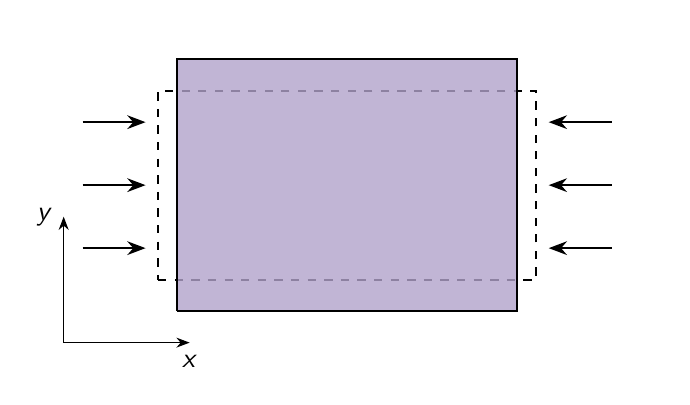
\begin{tikzpicture}[scale=0.8]
    %% Background
    \draw[draw=none] (-5,-3) to (5,-3) to (5,2.5) to (-5,2.5) to (-5,-3);
    %% Coordinate
    \draw[-Stealth] (-4.5,-2.5) to (-2.5,-2.5);
    \draw[-Stealth] (-4.5,-2.5) to (-4.5,-0.5);
    \draw
    (-2.5,-2.8) node{\(x\)}
    (-4.8,-0.5) node{\(y\)}
    ;
    %% Figure
    \draw[thick, dashed] (-3,-1.5) to (3,-1.5) to (3,1.5) to (-3,1.5) to (-3,-1.5);
    \draw[fill=square, fill opacity=0.8, thick] (-2.7,-2) to (2.7,-2) to (2.7,2) to (-2.7,2) to (-2.7,-2);
    %% Force
    \draw[thick, -Stealth] (-4.2,1) to (-3.2,1);
    \draw[thick, -Stealth] (-4.2,0) to (-3.2,0);
    \draw[thick, -Stealth] (-4.2,-1) to (-3.2,-1);
    \draw[thick, -Stealth] (4.2,1) to (3.2,1);
    \draw[thick, -Stealth] (4.2,0) to (3.2,0);
    \draw[thick, -Stealth] (4.2,-1) to (3.2,-1);
\end{tikzpicture}

\end{document}
